%%%%%%%%%%%%%%%%%%%%%%%%%%%%%%%%%%%%%%
% This poster uses a theme taken from Nathaniel Johnston
% http://www.nathanieljohnston.com/2009/08/latex-poster-template/
%%%%%%%%%%%%%%%%%%%%%%%%%%%%%%%%%%%%%%

\documentclass[final]{beamer}
\usepackage[scale=1.12]{beamerposter}
\usepackage{graphicx}
\usepackage{pstricks}
\usepackage{tikz}
\usepackage[french]{babel}
\usepackage{microtype}
\usepackage{default}
\usepackage{listings}
\usepackage[backend=biber]{biblatex}
\addbibresource{document.bib}
\renewcommand*{\bibfont}{\footnotesize}


%-----------------------------------------------------------
% Define the column width and poster size
% To set effective sepwid, onecolwid and twocolwid values, first choose how many columns you want and how much separation you want between columns
% The separation I chose is 0.024 and I want 4 columns
% Then set onecolwid to be (1-(4+1)*0.024)/4 = 0.22
% Set twocolwid to be 2*onecolwid + sepwid = 0.464
%-----------------------------------------------------------

\newlength{\sepwid}
\newlength{\onecolwid}
\newlength{\twocolwid}
\setlength{\paperwidth}{48in}
\setlength{\paperheight}{36in}
\setlength{\sepwid}{0.024\paperwidth}
\setlength{\onecolwid}{0.22\paperwidth}
\setlength{\twocolwid}{0.464\paperwidth}
\setlength{\topmargin}{-0.5in}
\usetheme{confposter}
\usepackage{exscale}

%-----------------------------------------------------------
% The next part fixes a problem with figure numbering. Thanks Nishan!
% When including a figure in your poster, be sure that the commands are typed in the following order:
% \begin{figure}
% \includegraphics[...]{...}
% \caption{...}
% \end{figure}
% That is, put the \caption after the \includegraphics
%-----------------------------------------------------------

\usecaptiontemplate{
\small
\structure{\insertcaptionname~\insertcaptionnumber:}
\insertcaption}

%-----------------------------------------------------------
% Define colours (see beamerthemeconfposter.sty to change these colour definitions)
%-----------------------------------------------------------

\setbeamercolor{block title}{fg=DarkGray,bg=white}
\setbeamercolor{block body}{fg=DarkGray,bg=white}
\setbeamercolor{block alerted title}{fg=DarkGray,bg=LightGray}
\setbeamercolor{block alerted body}{fg=DarkGray,bg=LightGray}
%-----------------------------------------------------------
% Name and authors of poster/paper/research
%-----------------------------------------------------------

\title{Techniques vidéo-ludiques pour logiciel auteur multimédia}
\author{Jean-Michaël Celerier}
\institute{Laboratoire Bordelais de Recherche en Informatique, Blue Yeti}

\begin{document}
\begin{frame}[fragile,t]    
   \setbeamerfont*{block title}{size=\Large,series=\bfseries}
\begin{columns}[t]
   \begin{column}{\sepwid}\end{column}
     \begin{column}{\onecolwid}
      \begin{block}{Problématique}
          \begin{columns}[t]
              \begin{column}{\onecolwid}\justify
                  Conception d'un logiciel d'écriture temporelle amené à être utilisé en production par des artistes tout en servant de plate-forme de recherche extensible pour des technologies multimédia.
                \end{column}
            \end{columns}        
      \end{block}
     \end{column}
     \begin{column}{\sepwid}\end{column}
     \begin{column}{\twocolwid}
         \begin{block}{Méthode}             
             \begin{columns}[t]	                 
                 \begin{column}{\onecolwid}\justify
                     Conception en entité-composant-système avec hiérarchies symétriques d'entités et de composants. 
                     Plusieurs moteurs opèrent en parallèle, avec une conception modulaire pour étendre le modèle.
                     \end{column}
                     \begin{column}{\onecolwid}\justify
                         Création d'entités sémantiques fortes par héritage, puis d'extensions faibles par composition.
                         Hiérarchie : création automatique de composants enfants à la création de nouvelles entités. 
                        \end{column}
                \end{columns}                 
            \end{block}
      \end{column}
      \begin{column}{\sepwid}\end{column}
      \begin{column}{\onecolwid}
          \begin{block}{Résultats}
          	\begin{columns}[t]
          		\begin{column}{\onecolwid}\justify
                      Plusieurs moteurs sont implémentés ainsi : moteur d'exécution, 
                      lecteur audio, réflection du système via une API réseau, interface graphique, 
                      moteur de gestion de contraintes à l'édition.
          		\end{column}
          	\end{columns}        
            \end{block}
        \end{column}         
   \begin{column}{\sepwid}\end{column}		
\end{columns}

\setbeamerfont*{block title}{size=\Large} 
  \vspace{0.5in}  
  \begin{columns}[t]
    
 \begin{column}{\sepwid}\end{column}
 
 \begin{column}{\onecolwid}
  \begin{beamercolorbox}[wd=\textwidth,colsep=0.05cm]{cboxb}\end{beamercolorbox}
 \end{column}
  
 \begin{column}{\sepwid}\end{column}
  
 \begin{column}{\twocolwid}
  \begin{beamercolorbox}[wd=\textwidth,colsep=0.05cm]{cboxb}\end{beamercolorbox}            
 \end{column}
  
 \begin{column}{\sepwid}\end{column}
 
 \begin{column}{\onecolwid}
  \begin{beamercolorbox}[wd=\textwidth,colsep=0.05cm]{cboxb}\end{beamercolorbox}
 \end{column}         
  
 \begin{column}{\sepwid}\end{column}
\end{columns}
  \vspace{-1ex}  
  \begin{columns}[t]
    \begin{column}{\sepwid}\end{column}
    \begin{column}{\onecolwid}
      \vskip2ex
       \begin{block}{Partitions interactives}
\begin{figure}
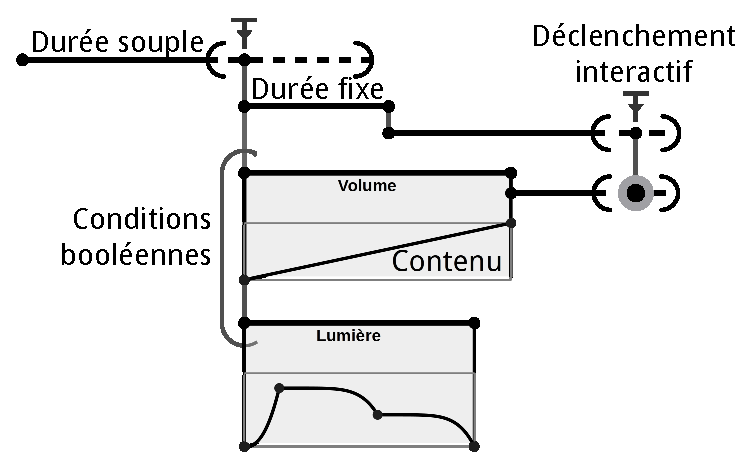
\includegraphics[width=\columnwidth]{images/score.eps}
\caption{Syntaxe d'une partition interactive}
\end{figure}
Autres approches:  Antescofo, INscore, OpenMusic, environnements de programmation (Tuiles réactives).

Application : musique, scénographie, contrôle de robots
\end{block}
      \vskip2ex
      \begin{block}{Modèles pour logiciels auteurs}
Standard : modèle-vue-contrôleur, modèle-vue-présenteur, document-présentation-instrument, modèle-vue-modèle de vue, présentation-abstraction-contrôle, programmation fonctionnelle réactive.
Donnent des responsabilités à différents éléments de l'application et spécifient la communication entre ces éléments et la manière dont une interaction utilisateur affecte le modèle de données.
Principalement orienté pour l'affichage, mais s'adaptent peu à d'autres moadlités.

Problématique de l'édition; c.f. Object-Oriented Programming for Graphics

\end{block}
    \end{column}

    \begin{column}{\sepwid}\end{column}
    \begin{column}{\twocolwid}
      \begin{columns}[t,totalwidth=\twocolwid]
        \begin{column}{\onecolwid}\vspace{-.67in}
            \vskip2ex
            
        	\begin{block}{Édition en temps réel avec rollback}
                
        	\end{block}
        \end{column}
        \begin{column}{\onecolwid}\vspace{-.67in}
            \vskip2ex
            \begin{block}{Implémentation}
Système d'entités adapté pour \textbf{hiérarchie fixée} dans le modèle : tout ne se compose pas avec tout.
Identification unique fortement typée avec cache~: 
\begin{itemize}
    \item Dans un document par chemins : nécessaire pour gestion undo - redo et identification sur réseau.
    Pattern Commande réparti pour \textbf{édition multi-utilisateurs}.
    \item À un niveau de hiérarchie donnée : performance pour itération.
   \end{itemize}

Création de familles de composants fortement ou faiblement typés selon le besoin, et associés à un élément de modèle : fig.~\ref{fig.uml}.

Contrairement à moteurs de jeu, \textbf{pas de synchro des tick rate} car tous les systèmes sont séparés ; certains systèmes peuvent fonctionner sur le même thread ou sur des threads différents. 
Les systèmes peuvent communiquer entre eux.
\end{block}
        \end{column}
      \end{columns}
      \vskip2.5ex
      \begin{block}{}
          \begin{figure}
              \centering
              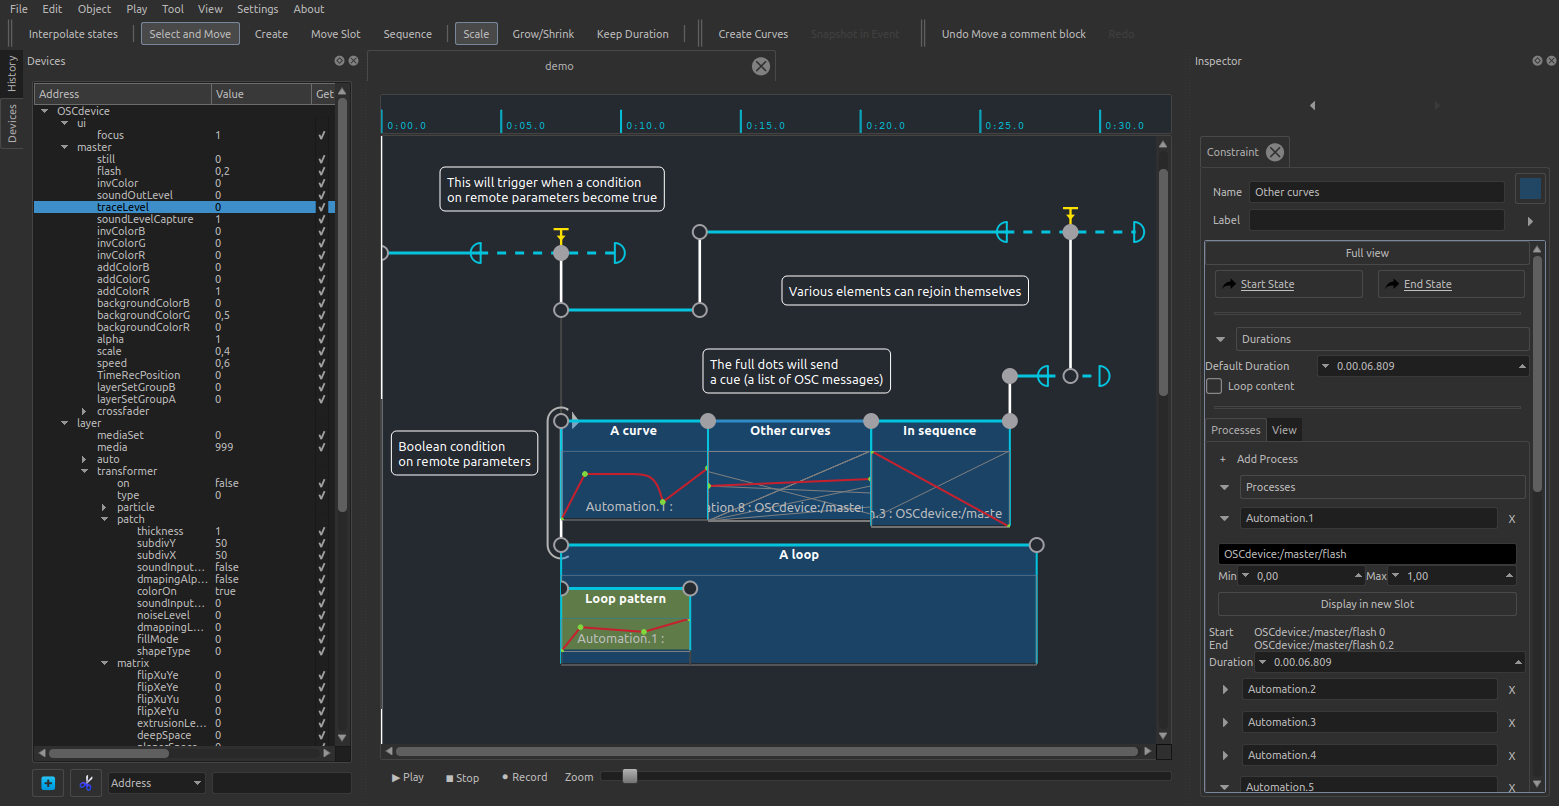
\includegraphics[width=\textwidth]{images/iscore.png}
              \caption{Un scénario d'exemple i-score}
            \end{figure}
      \end{block}
  \end{column}
  \begin{column}{\sepwid}\end{column}
  \begin{column}{\onecolwid}
    \vskip2ex
    \begin{block}{}
    \vspace{-3cm}
    \begin{figure}\centering
        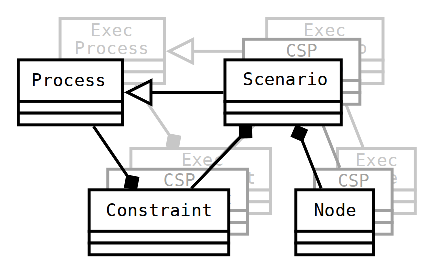
\includegraphics[width=0.7\columnwidth]{images/orga3.eps}
        \caption{Organisation des graphes d'entités - composants}
        \label{fig.uml}
    \end{figure}
\end{block}
\begin{block}{Prochaines étapes}
    \small
    \begin{itemize}
        %\item Scripting intégré : intégration d'un langage de haut-niveau interprété (\textbf{QML}) pour prototyper plus simplement sur le logiciel.
        \item Implémentation audio plus poussée via \textbf{libaudiostream}\cite{letz_specification_2014} qui crée un graphe semblable à celui d'i-score.
        \item Travail en cours sur modèles et \textbf{processus spatiaux} : écriture avec des données multi-dimensionnelles.
    \end{itemize}
\end{block}
    \vskip2ex
    \begin{block}{Informations complémentaires}
    	% Site web
    	% Article
      {Articles:
      \begin{itemize}
        \item Modèles formels sur lesquels se base i-score~:~\\\cite{allombert_system_2007,arias_modelling_2014}.
        \item Paradigme graphique OSSIA~:~\cite{celerier_ossia:_2015}.
      \end{itemize}
      \vspace{0.1in}\noindent i-score peut être téléchargé librement sur
      \begin{itemize}
        \item \url{www.i-score.org}
      \end{itemize}}
\end{block}
    \vskip2ex
    \begin{block}{Références}
        \footnotesize\printbibliography
    \end{block}
    \vskip2ex
  \end{column}
  \begin{column}{\sepwid}\end{column}			% empty spacer column
 \end{columns}
\end{frame}
\end{document}

